\subsubsection{Arduino}
Arduino is a company producing electronic boards for the purpose of reading some input (e.g. from a connected sensor), and then turn this into some output (e.g. a motor or an LED).
The decision depends on the program the user creates and implements on the Arduino board \cite{arduino_arduino_nodate}.
The board exists in several configurations depending on the needs, of which only the Arduino Uno and the Arduino Mega are available for us to use in this project \cite{arduino_arduino_products}.

\begin{figure}[H]
  \centering
  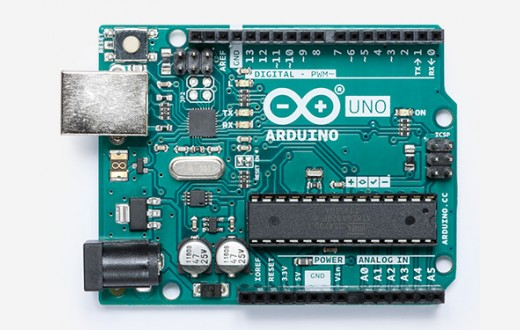
\includegraphics[width=4cm]{images/techAnalysis/ArduinoUno.jpg}
  \caption{Arduino Uno Rev3 \cite{Arduino-figure-UNO}}\label{fig:sssec:arduino-Uno}
\end{figure}
The Arduino Uno, seen in \autoref{fig:sssec:arduino-Uno}, is an entry level board in the Arduino universe, it features a clock speed of 16Mhz, 2KB RAM and 32KB flash memory.
The communication with sensors, motors and other components is done through the boards digital input/output pins, which this board has 14 of, or through the 6 analog pins.
The board can be connected to a computer through its USB port.
The board is powered through an adapter at recommended 7v to 12v, depending on which and how many components that are connected, or can be powered through the USB port. \cite{arduino_arduino_UNO}

\begin{figure}[H]
  \centering
  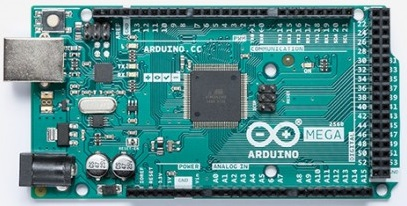
\includegraphics[width=4cm]{images/techAnalysis/ArduinoMega.jpg}
  \caption{Arduino Mega 2560 Rev3 \cite{Arduino-figure-MEGA}}\label{fig:sssec:arduino-Mega}
\end{figure}
The Arduino Mega, which can be seen in \autoref{fig:sssec:arduino-Mega}, when compared to the Arduino Uno, is a more powerful board with more options.
Like the Arduino Uno, the Arduino Mega is powered at 16MHz clock speed, but it features 8KB RAM and 256KB flash memory.
The board provides more options with it's 54 digital I/O pins, and 16 analog pins.
And, like the Arduino Uno, the board can be connected to a computer through its USB.
Like the Arduino Uno the Arduino Mega can be powered by either a adapter, or by the USB port. \cite{arduino_arduino_MEGA}
